Für dieses Seminar haben wir einen Prototypen, der die Implementierung eines der von uns vorgeschlagenen Integer Linear Programs mit einem Editor-Frontend vereint, entwickelt. Diesen möchten wir im Folgenden vorstellen.

\subsection{User Interface}

In diesem Abschnitt wird die grafische Oberfläche, welche Teil des Prototypen ist, mit ihren
Funktionalitäten vorgestellt. Außerdem wird die Bedeutung für einen eigenen Editor im
Rahmen des Seminars erläutert.

\subsubsection{Beschreibung}

Die GUI ist eine Webanwendung, welche mit Javascript programmiert wurde. Hierzu wurden
die Javascript-Bibliotheken Cytoscape.js\cite{cytoscape} und Angular.js\cite{angularjs} benutzt. Cytoscape.js bietet bereits
Funktionalitäten, um einen Graphen darzustellen und zu manipulieren. Angular.js wurde als
Javascript Framework benutzt, um die Interaktion mit Html und Javascript zu erleichtern.
Ansonsten wurde reines Javascript benutzt, um die weiteren Features zu implementieren.

Da diese Arbeit sich auf das inkrementelle Einfügen von Knoten fokussiert, wurde der Editor
mit einer Funktion ausgestattet, welche es erlaubt, einen Knoten lediglich mit ein paar
Mausklicks einzufügen und die Größe festlegen zu können. Es wird verhindert, dass ein neu
eingefügter Knoten mit einem bestehenden Knoten überlappt, indem für den neuen Knoten
genug Platz geschaffen wird. Der Algorithmus um Platz zu schaffen unterstützt die vier
folgenden Modi:

\begin{itemize}
	\item es wird Platz gemacht, indem alle Knoten in eine der vier orthogonalen Richtungen
verschoben werden, damit unmittelbar links, rechts, oberhalb und unterhalb von dem
neuen Knoten kein anderer Knoten sich befindet. Alle Knoten, die in die gleiche
Richtung verschoben werden, werden um den gleichen Betrag verschoben. Dieser
Betrag wird so bestimmt, dass alle Knoten einen minimalen Abstand von dem
eingefügten Knoten einhalten.
	\item der erste Modus aber es wird nur links und rechts Platz gemacht.
	\item der erste Modus aber es wird nur oben und unten Platz gemacht.
	\item die Knoten werden um den gleichen Betrag nach außen verschoben, damit kein
anderer Knoten mit dem Neuen überlappt
\end{itemize}

In jedem Modus wird ein Mindestabstand zwischen dem neu eingefügten Knoten und allen
anderen eingehalten. Somit kommt es zu keinen Überlappungen der Knoten, die zu nah
beieinander sind. Abhängig vom Modus der gerade aktiv ist zeigt die GUI ein entsprechendes
Overlay um anzuzeigen, wo überall Platz gemacht wird. Nachdem ein Knoten mit einem der
vier Modi eingefügt wurde, kann dessen Größe festgelegt werden. Anschließend hat der
Benutzer die Möglichkeit über einen Button das Layout des Graphen anzupassen. Somit wird
der Platz, der vorher gemacht wurde, wieder minimiert, wobei versucht wird, gewisse
Layoutbedingungen nicht zu verletzen (die wird näher in FIXME beschrieben).
Des Weiteren zeigt jeder Knoten einen Titel und eine Beschreibung an. Somit können
Informationen von Thesen und Argumenten in den Knoten angezeigt werden. Dies ist eine
grundlegende Anforderung an eine Argumentkarte.

Außerdem können Knoten horizontal sowie vertikal auf einer Linie angeordnet werden. Dies
hilft dem Benutzer, den Graphen nach seinen Bedürfnissen zu gestalten. Hier können
verschiedene Funktionen genutzt werden, um neue Position der Knoten zu berechnen. In
dem Prototypen wird der Mittelwert der $x$- oder $y$- Koordinate berechnet und als neue Position
der auszurichtenden Knoten benutzt. Eine weitere Funktion könnte die Knoten an dem zuletzt
markierten Knoten ausrichten oder an einem Knoten ausrichten, den man explizit auswählt.
Da es sich nur um einen Prototypen handelt wurden diese Funktionen jedoch nicht
implementiert.

Die letzte wichtige Funktion ist das Importieren von \textit{.graphml} Dateien. Somit können
Argumentkarten aus dem Argunet-Editor importiert werden. Dies erlaubt ein schnelles Testen
der Algorithmen. Es werden Position und Größe der Knoten, Kanten zwischen den Knoten
und die Beschriftung der Knoten importiert. Falls man ein orthogonales Kantenrouting
implementiert hätte, könnte man hier auch noch die Position der Knicke auf den Kanten
importieren, falls diese in der \textit{.graphml}-Datei vorhanden sind.

\subsubsection{Bedeutung für das Seminar}

Die Anforderung der Philosophiestudenten war, dass der Graph sich nur wenig ändern sollte,
wenn ein Knoten eingefügt wird. Die verschiedenen Modi dienen dazu, dass der Benutzer
entscheiden kann, wieviel sich im Graphen ändert. Hier muss angemerkt werden, dass nur
der erste Modus garantieren kann, dass sich orthogonale Kanten nicht überlappen würden.
Da diese Arbeit sich jedoch ausschließlich auf die Position der Knoten bezieht und die Kanten
ausklammert, wird dieses Problem nicht weiter diskutiert.

Der anschließende Layoutalgorithmus versucht dann so weit es geht das ursprüngliche
Layout wieder herzustellen. Wie ähnlich der Graph nach dem Einfügen des Knoten aussieht,
hängt stark von der Position und der Größe des neuen Knoten ab. Die zusätzliche
Ausrichtfunktion dient dazu, dass der Benutzer in das Layout eingreifen kann, und noch mehr
mitbestimmen kann wie das endgültige Layout aussieht.

Diese beiden Funktionen sind sinnvoll, da der Benutzer, welcher eine Argumentkarte erstellt,
meistens bereits weiß, wie die Knoten angeordnet werden sollen. Insbesondere weiß der
Benutzer auch wie ein neu eingefügter Knoten positioniert werden soll. Der Benutzer ist
jedoch nicht darauf angewiesen diese Layoutfunktionen zu benutzen. Ohne eine Anpassung
vom Benutzer versucht der ILP-Algorithmus eine optimale (und somit in den meisten Fällen
eine für den Benutzer wünschenswerte) Lösung zu finden.
 Die GUI bietet dem Benutzer Funktionen um schnell einen Graphen inkremetell aufzubauen
und zugleich hat er die Freiheit selbst mit zu entscheiden, wie er den Graphen gestaltet.



\subsection{Backend}

Das Backend hat vor allem die Aufgabe, nach einer erfolgten Einfügung ein neues Layout zu berechnen, welches die zu Beginn dieser Arbeit vorgestellte Optimierungsfunktion \ref{eqn:opt:complete} in gewissem Rahmen optimiert. Hierfür haben wir das in Abschnitt \ref{sub:ilp:2} vorgestellte ILP, das Vertauschungen von Knoten in begrenztem Maße zulässt, mit einigen Anpassungen implementiert.

Beim Backend haben wir auf eine Implementierung in Python unter Zuhilfenahme des Django-Webframeworks\cite{django} gesetzt, die mit der GUI über Ajax kommuniziert. Für die Lösung des ILPs kommt Gurobi\cite{gurobi} zum Einsatz.

\subsubsection{Abweichungen vom beschriebenen ILP}
\label{sub:impl:opt}

Zunächst haben wir wie in Abschnitt \ref{sub:ilp:2} schon angedeutet versucht, die Anzahl der Bedingungen, die für Überlappungsfreiheit sorgen werden, auf eine sub-quadratische Anzahl zu senken. Eine hilfreiche Beobachtung ist hier, dass viele dieser Bedingungen nicht benötigt werden, da die entsprechenden Knoten aufgrund des Abstands zueinander im Ausgangslayout sowieso nicht überlappen werden. Wir fügen daher dem ILP anfangs nur entsprechende Bedingungen für adjazente Knoten hinzu, und werden weitere Bedingungen nur dann ins ILP aufnehmen, wenn sie benötigt werden. Unser erster Ansatz war hier, die Callback-Funktionalität von Gurobi zu nutzen. Dies erwies sich allerdings als unnötig aufwändig, da diese Callbacks teilweise nur unter sehr speziellen Bedingungen aufgerufen werden. Eine einfachere und effiziente Lösung ist es, nach Lösung des ILPs durch Gurobi alle Knoten auf Überlappungen zu testen, bei Bedarf neue Bedingungen einzufügen und das bereits gelöste, aber veränderte Modell von Gurobi erneut lösen zu lassen. Im Normalfall ist eine neue Lösung, die die zusätzlichen Bedingungen berücksichtig, dann in sehr kurzer Zeit gefunden. Dies wiederholen wir so lange, bis keine Überlappungen mehr auftreten. In unseren Tests sind im Normalfall nicht mehr als eine oder zwei Wiederholungen nötig gewesen.

Eine weitere Besonderheit ist, dass wir für die Vektor-Vektor-Abstände, wie sie z.B. in der Optimierungsfunktion \ref{eqn:opt:complete} vorkommen, die 1-Norm statt der intuitiv vielleicht sinnvolleren 2-Norm verwendet haben. Dies hat den Grund, dass sich die 2-Norm in einem Integer \textit{Linear} Program nicht abbilden lässt. Es wäre an dieser Stelle zwar möglich ein Integer \textit{Quadratic} Program stattdessen aufzustellen (und von Gurobi lösen zu lassen), allerdings wollten wir die Komplexität zunächst auf ein ILP beschränken.

Des Weiteren haben wir zusätzlich eine Klasse von Bedingungen eingebaut, die es ermöglicht, mehrere Knoten auf dieselbe $x$- oder $y$-Koordinate zu zwingen. Dies ist vor allem auf den in Abschnitt \ref{sub:tasks} angesprochenen Wunsch zurückzuführen, mehrere Knoten aneinander "`ausrichten"' zu können.

Eine weitere Optimierung, die die Zeit, die zum Lösen des Systems stark senkt, ist, dass wir die Positionen aller Knoten im Ausgangslayout an die von Gurobi verwendeten Heuristiken zum Finden einer Startlösung übergeben.

\subsection{Ergebnisse}

Wir haben den von uns entwickelten Prototypen mit einigen bereitgestellten GraphML-Dateien getestet. Die Instanzen hatten eher kleine Größen von ca. 20 Knoten. Auf diesen Instanzen wurde das ILP von Gurobi nahezu in Echtzeit gelöst.

\begin{figure}
	\begin{center}
		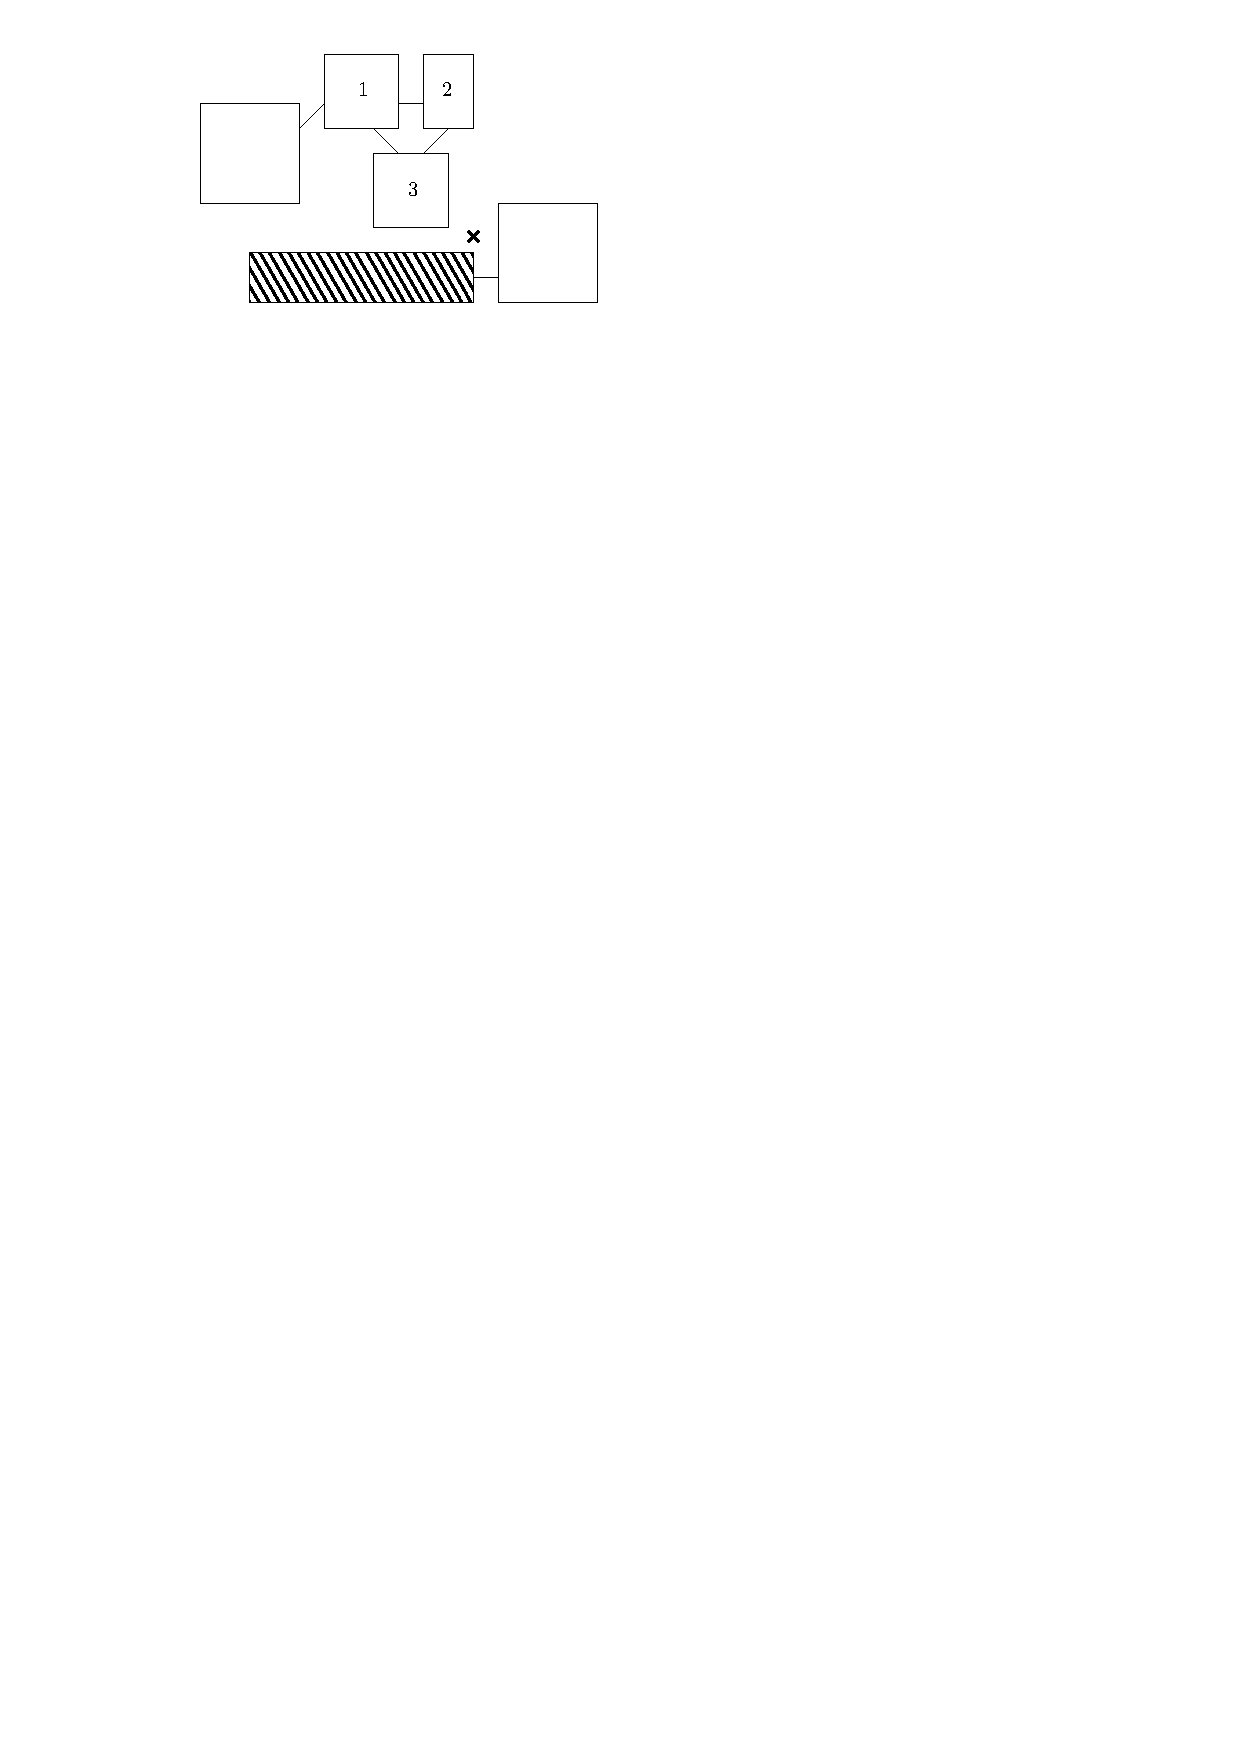
\includegraphics{figures/order.pdf}
		\caption{Problematische Einfügung}
		\label{fig:order-too-strict}
	\end{center}
\end{figure}

Die wichtigste Beobachtung ist, dass die Einschränkung, nur direkt benachbarte Paare von Knoten tauschen zu dürfen, für realistische Instanzgrößen unpraktikabel ist. Am Beispiel von Abbildung \ref{fig:order-too-strict} wird dies deutlich: Der schraffierte Knoten sollte an der Position, die durch das Kreuz angezeigt wird, eingefügt werden. Die Position, an der der schraffierte Knoten jetzt gezeichnet wurde, wäre vermutlich eine gute Wahl. Um hier platziert zu werden, müsste er allerdings (relativ zu der Position des Kreuzes und der links-oberen Ecken der Knoten) in der horizontalen Reihenfolge die Positionen mit den Knoten $1, 2$ und $3$ tauschen, was in diesem eingeschränkten Modell nicht möglich ist. Dieses Problem wird umso ausgeprägter, je größer die Instanzen werden. TODO mehr dazu

Beobachtet haben wir außerdem, dass der neu eingefügte Knoten unserem Gefühl nach häufig zu weit von der Position, an der man ihn hat einfügen wollen, platziert wurde. Außerdem wurde unserem Gefühl nach die Möglichkeit der Skalierung gegenüber der Verschiebung von Knoten (siehe Abschnitt \ref{par:scale}) zu intensiv genutzt wurde. Dies ist zurückzuführen auf die Wahl der Konstanten $\alpha, \beta$ und $\gamma$ in der Optimierungsfunktion \ref{eqn:opt:complete}.



TODO größere Instanzen?
